\documentclass[letterpaper,12pt]{article}
\author{Kiyo Akabori}
\title{Transmission Experiment on the Ripple Phase}
%-------------------------------------Package-----------------------
\usepackage{graphicx}
\usepackage{tabularx}
\usepackage[lofdepth,lotdepth]{subfig}%subfloat
\usepackage{bm}%bold math
\usepackage{color}
\usepackage[centertags]{amsmath}
\usepackage{mathrsfs}
\usepackage{amsmath,amssymb}
\usepackage{amsfonts}
\usepackage{amssymb}
\usepackage{amsthm}
\usepackage{newlfont}
\usepackage{epstopdf}
%------------------------------new command------------------------
\newcommand{\dg}{$^{\circ}$}%degree symbol
\newcommand{\iang}{\AA$^{-1}$}%inverse Angstrom symbol
\newcommand{\motor}{$\theta_m$}%motor angle

%\setlength{\oddsidemargin}{0cm} \setlength{\topmargin}{0cm}
%\setlength{\textheight}{22cm} \setlength{\textwidth}{16cm}
%-----------------------------------------------------------------

\begin{document}
\title{Ripple Phase}
\author{Kiyo Akabori}
\today

\tableofcontents
\listoffigures
\listoftables

\newpage
\section{Notation}
\begin{itemize}
\item color scale of intensity profile: [minimum maximum]
\item $\theta$: Bragg angle or usual $\theta$ in spherical coordinates
\item $\phi$: usual $\phi$ in spherical cooridnates
\item $\omega$: angle of incidence
\item $\theta_m$: motor angle
\item $\hat{\theta}$: angle measured from equator in q-space
\item $S$, S-distance: distance between the center of a sample and the CCD screen
\item $D$, D-spacing: repeat spacing of lipid bilayers
\item $d$, d-spacing: distance between lipid chains
\item $p_x$: pixel number in horizontal direction
\item $p_z$: pixel number in vertical direction
\item $\theta_t$: chain tilt angle
\item $\gamma$: $\gamma$ angle of ripple phase [refer to Figure \ref{fig:Sun1996}]
\item $\xi$: the angle between the midplane of the major side and the ripple direction
\item X-axis: horizontal axis through the beam in the CCD frame
\item Z-axis: vertical axis through the beam in the CCD frame
\item (X,Z): position on the CCD detector with respect to the beam
\end{itemize}

\newpage
\section{Overview of the Experiment}
Figure \ref{fig:holderdrawing1} is a schematic drawing of the sample holder, showing its dimensions. The axis of motor (axis of rotation) does not coincide with the center of the sample; rather, the sample is 21.10 mm above the axis. The axis of the motor is 1 mm above the surface of Peltier, which corresponds to the thickness of a silicon wafer. The thickness of the sample is exaggerated in the figure. Figure \ref{fig:holderdrawing2} is a picture showing schematically the sample holder and sample at the transmission angle. 
%-----------schematic drawings of the sample holder----------------
\begin{figure}[htbp]
	\centering
	\subfloat[Side view of holder with its dimensions][Side view of holder with its dimensions. A sample (lipids and a glass cover slip) is shown by a blue rectangle.]{
	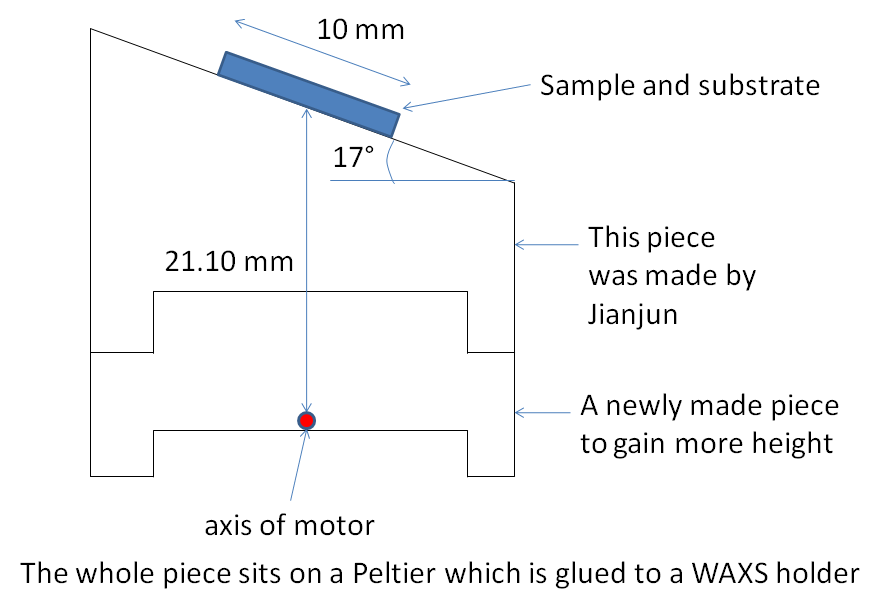
\includegraphics[width=0.5\textwidth]{holderdrawing1}
	\label{fig:holderdrawing1}}
	\qquad
	\subfloat[Side and top views of the holder at the transmission angle][Side and top views of the holder at the tranmission angle showing how the beam (yellow arrow) hits the sample.]{
	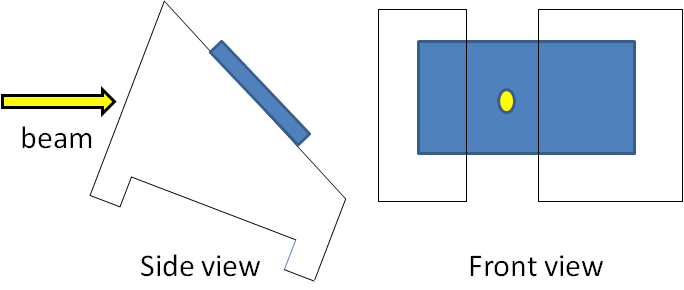
\includegraphics[width=0.5\textwidth]{holderdrawing2}
	\label{fig:holderdrawing2}}
	\caption{Schematic drawings of the sample holder used in transmission experiments.}
\end{figure}
%-------------------------------------------------------

Pictures of the sample holder are shown in Figure \ref{fig:SampleHolder}. A piece of lead tape is attached to the back of the holder in order to block air scattering before the beam hits the sample. A small window is cut in the tape so that the beam does not get blocked. There is also a groove in the metal piece as a pathway for the beam at the transmission angle.
%-----------------Pictures of the sample holder----------
\begin{figure}[htbp]
	\centering
	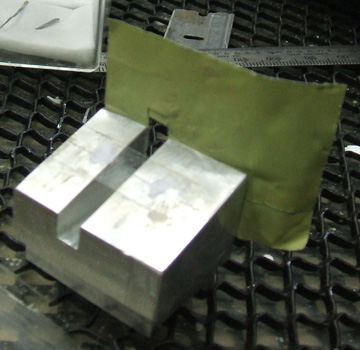
\includegraphics[width=0.3\textwidth]{SampleHolder1}
	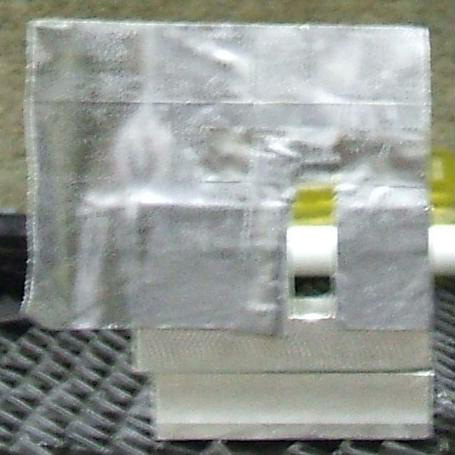
\includegraphics[width=0.3\textwidth]{SampleHolder2}
	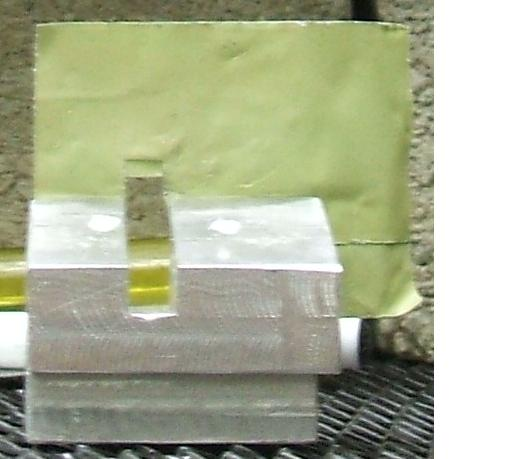
\includegraphics[width=0.3\textwidth]{SampleHolder3}
	\caption[Pictures of the sample holder used in transmission experiments]{Pictures of the sample holder used in transmission experiments. (left) Looking down on the holder. (middle) Looking downstream. (right) Looking upstream.}
	\label{fig:SampleHolder}
\end{figure}
%--------------------------------------------------------------------

Figure \ref{fig:chamber} shows the sample holder at three different motor angles denoted by $\theta_m$ in a transmission experiment. $\theta_m$ is set to 0\dg\,before the holder is removed from the chamber. At \motor\ = 17\dg, the sample is level. We will call $\theta_m$ between $17$\dg\,and 22\dg\, glancing angles. D-spacings are measured at a fixed glancing angle between 18\dg\, and 22\dg. After measurements of the D-spacing of a sample, $\theta_m$ is set to $-28$\dg\ to obtain transmission data. When $\theta_m$ is set to $-28$\dg, the angle of incidence, $\omega$, becomes 45\dg. We will call this motor angle the transmission angle. Experimental details are covered in the following sections.
%---------------pictures of the sample holder in chamber-----------
\begin{figure}[htbp]
	\centering
	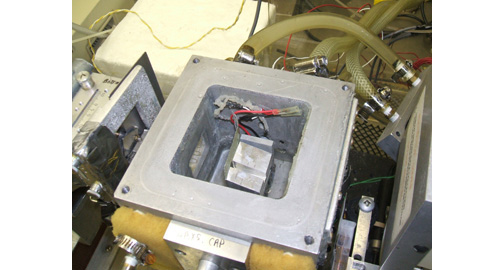
\includegraphics[width=0.8\textwidth]{chamber1}
	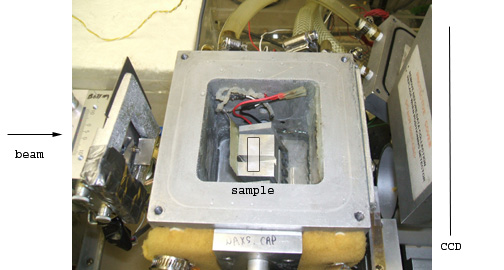
\includegraphics[width=0.8\textwidth]{chamber2}
	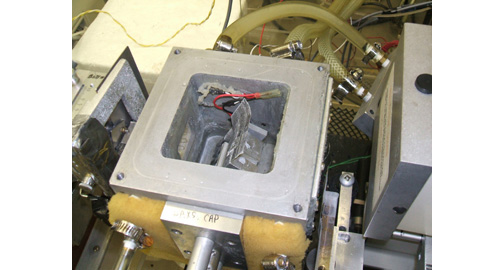
\includegraphics[width=0.8\textwidth]{chamber3}
	\caption[Topview pictures of the sample holder in the hydration chamber]{Topview pictures of the sample holder in the hydration chamber. From top to bottom, \motor\ = 0\dg\ or $\omega=17$\dg, \motor\ = 17\dg\ or $\omega=0$\dg, and \motor\ = $-28$\dg or $\omega=45$\dg. The beam comes from the left hand side. The CCD is located at the right hand side.}
	\label{fig:chamber}
\end{figure}
%---------------------------------------------------------------------

Figure \ref{fig:ChamberGeometry} is a diagram showing geometry of the setup. As shown in the diagram, the region between the shutter and the first mylar window is R0, between the first and second mylar is R1, between the second mylar and the sample is R2, between the sample and the third window is R3, between the third and fourth window is R4, and the region beyond the beam stop is R5. Note that the distance between the center of the chamber and CCD is 116.1 mm, which is measured using a silver behenate sample on a silicon wafer by rotating it. As noted earlier, the center of the sample will depend on \motor\ in transmission experiment. When helium is used, R1, R2, R3, and R4 are filled with helium. R0 and R5 are always filled with air molecules.
%-------------Topview diagram of the setup----------------------
\begin{figure}[htbp]
	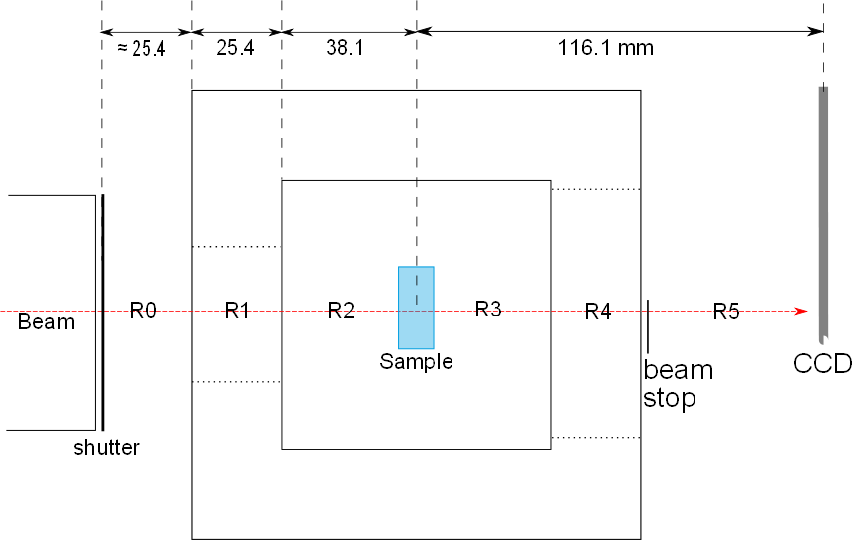
\includegraphics[width=\textwidth]{ChamberGeometry}
	\caption[A topview diagram of the setup]{A topview diagram of the setup. Lengths are all in units of mm. The entrance and exit windows of the chamber are shown by dots.}
	\label{fig:ChamberGeometry}
\end{figure}
%---------------------------------------------------------------------

Figure \ref{fig:beam} shows the beam that was used. 
\begin{figure}[htbp]
	\subfloat[][Beam profile in $q_r$]{	
		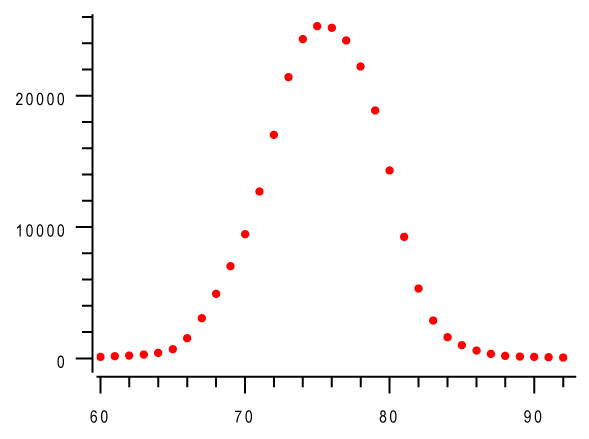
\includegraphics[width=0.5\textwidth]{beam_qr}}
	\subfloat[][Beam profile in $q_z$]{
		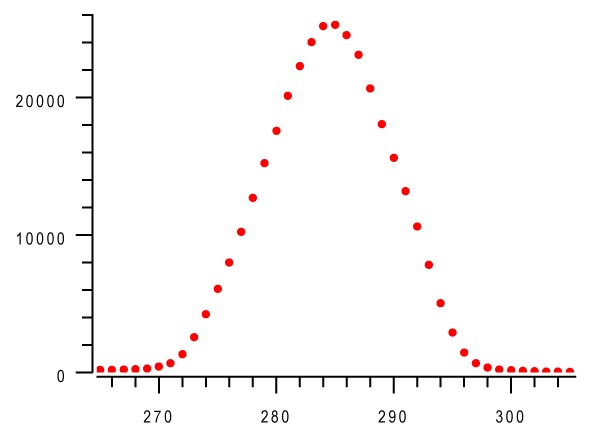
\includegraphics[width=0.5\textwidth]{beam_qz}}
	\caption[The beam profile]{The beam profile. The beam height = 0.88 mm. The width = 0.61 mm.}
	\label{fig:beam}
\end{figure}
%---------------------------------------------------------------------
The CCD detector size is 70 mm by 70 mm. Its pixel size is 0.068 mm per pixel. The wavelength of the beam is 1.5418 \AA. The lipid used is dimyristoylphosphatidylcholine (DMPC) spread as an approximately $10\mathrm{\mu m}$ film from a mixture of chloroform: methanol 1:1 with the rock and roll procedure on a $75\mathrm{\mu m}$-thick glass coverslip. When the color scale of intensity map is written as [minimum maximum] in gray scale, pixels with intensity greater than 150 are all white and those with intensity less than 0 are all black. The dynamic range of the CCD detector is about 65,000.

\newpage
\section{Leveling of Samples}
Before a sample-to-CCD distance, or S-distance, can be measured, a silver behenate (AgBeh) sample must be levelled accurately. Because the substrate is a thin glass coverslip whose thickness is only $75\,\mathrm{\mu m}$, which sits above a groove, cutting of the beam by the substrate cannot be used to determine if a sample is level. Instead, sample scattering is used to level the sample. If the angle of incidence is negative, the beam is absorbed by the substrate before it reaches the sample. The path length of the beam inside the substrate is given by $75\,\mathrm{\mu m}$/$\sin |\omega|$. So, at small $\omega$ such as $-0.1$\dg, absorption of the beam is significant. In contrast, at a positive angle of incidence, lamellar peaks are observed on the meridian [See Figure \ref{fig:Leveling}]. By changing the angle of incidence, $\omega$, from small negative values to positive ones (usually, around $-0.5$\dg\ to $0.5$\dg) in an increment of 0.1\dg, leveling of a sample can be accomplished. 
%---------------------------------------------------------------------
\begin{figure}[htbp]
	\centering
	\subfloat[][$\omega$ = $-0.1$\dg]{
		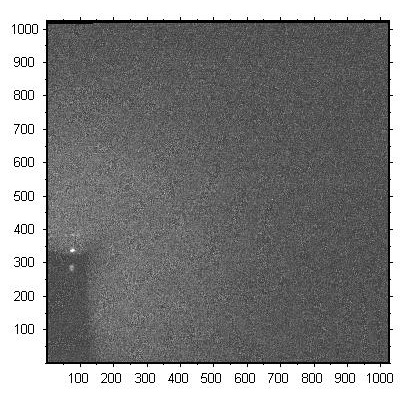
\includegraphics[width=0.5\textwidth]{leveling_np1}}
	\subfloat[][$\omega$ = 0\dg]{
		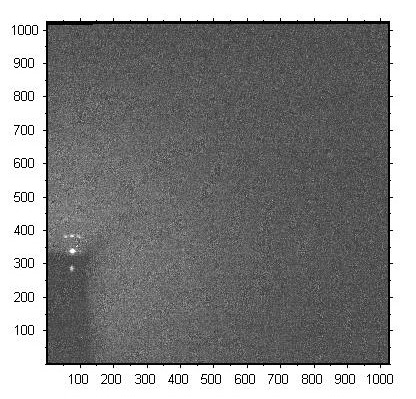
\includegraphics[width=0.5\textwidth]{leveling_0}}

	\subfloat[][$\omega$ = 0.1\dg]{
		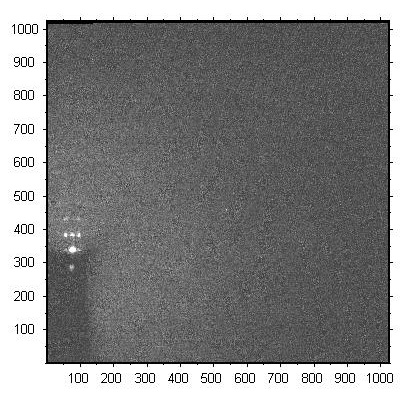
\includegraphics[width=0.5\textwidth]{leveling_pp1}}
	\subfloat[][$\omega$ = 0.2\dg]{
		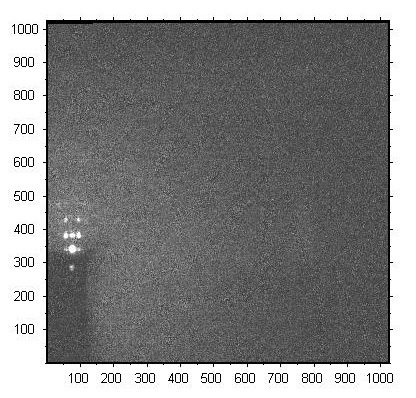
\includegraphics[width=0.5\textwidth]{leveling_pp2}}
	\caption[Leveling: 10 seconds]{Diffraction from ripple phase DMPC at grazing angles , that is, $|\omega|$ less than the critical angle, to show how lamellar-peak intensities change at different angles. Exposure time was 10 seconds. The sample-to-detector distance is 121.6 mm.}
	\label{fig:Leveling}
\end{figure}
%---------------------------------------------------------------------

A caveat here is that even at negative $\omega$, weak Bragg peaks are usually observed on the meridian although the beam should be absorbed by the substrate at negative angles. (Perhaps because the thickness of the sample is $10\,\mathrm{\mu m}$ so some parts of it is actually exposed to the beam at small negative angles? Need to investigate this point...) In order to overcome this issue, the intensity of WAXS peak is used to accurately level the sample. Since the critical angle of lipid samples is approximately 0.17\dg\ at wavelength of 1.5418 \AA, the intensity of wide-angle peak becomes much stronger when $\omega$ is changed from 0.1\dg\ to 0.2\dg\ as seen in Figure \ref{fig:CriticalAngle}. So, the usual protocol to level a sample is to scan from supposedly a negative $\omega$ with a short exposure time, say 10 seconds, until lamellar peaks become reasonable strong, and then take longer shots (30 seconds) at angles that are guessed to be 0\dg, 0.1\dg, and 0.2\dg to see a big change in WAXS-peak intensity. (One may also take shots at 0.3\dg\ and 0.4\dg\ to confirm that WAXS-peak intensity does not change significantly from 0.2\dg\ to 0.4\dg.)
%---------------------------------------------------------------------
\begin{figure}[htbp]
	\centering
	\subfloat[][$\omega$ = 0\dg]{
		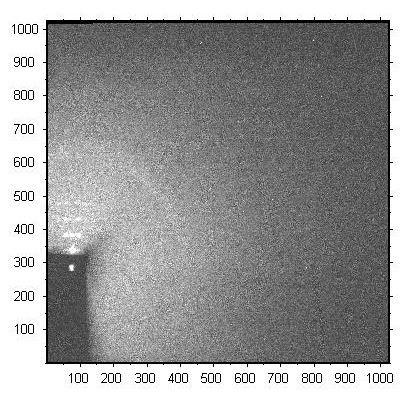
\includegraphics[width=0.5\textwidth]{leveling_0_1}}
	\subfloat[][$\omega$ = 0.1\dg]{
		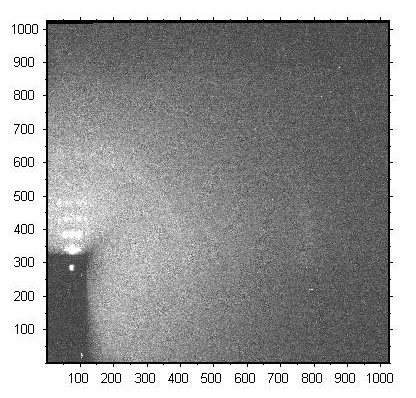
\includegraphics[width=0.5\textwidth]{leveling_pp1_1}}
	
	\subfloat[][$\omega$ = 0.2\dg]{
	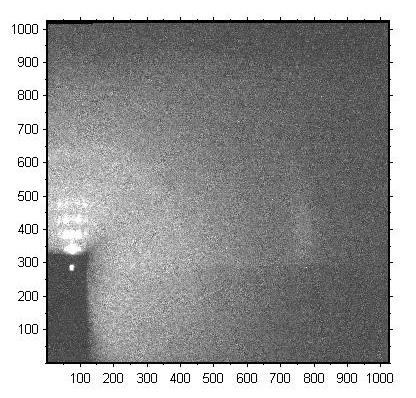
\includegraphics[width=0.5\textwidth]{leveling_pp2_1}}
	\caption[Leveling: 30 seconds]{Diffraction from ripple phase DMPC at grazing angles. Exposure time was 30 seconds. WAXS peak is almost invisible at $\omega$ = 0\dg. Note an increase in WAXS peak intensity when \motor\ is increased from 0.1\dg\ to 0.2\dg. The color scale is the same as in Figure \ref{fig:Leveling}.}
	\label{fig:CriticalAngle}
\end{figure}
%---------------------------------------------------------------------

\newpage
\section{Measurements of s-distance}
S-distance is the distance between the center of the sample and the CCD screen. After a AgBeh sample is leveled, the S-distance is measured at a glancing angle. As noted in the Overview of Experiment section, the center of sample does not coincide with the motor axis. This offset causes the S-distance to change as samples are rotated, which makes the usual method of rotation to measure an s-distance inappropriate. To overcome this problem, mosaic spread of a sample is utilized. Because of sample mosaicity, many Bragg orders are observed even at a fixed angle. Then, the positions of these peaks are fitted in the ds program to determine the S-distance [See Figure \ref{fig:AgBeh22deg}]. 
%------------------------------------------------------------------
\begin{figure}[htbp]
	\centering
	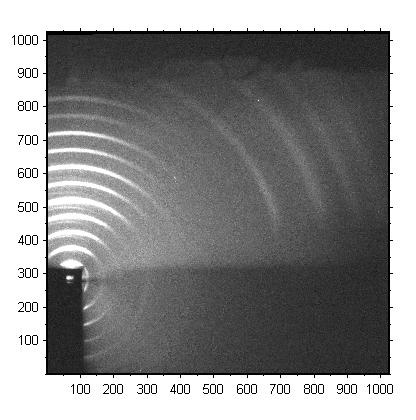
\includegraphics[width=0.45\textwidth]{AgBeh_22}
	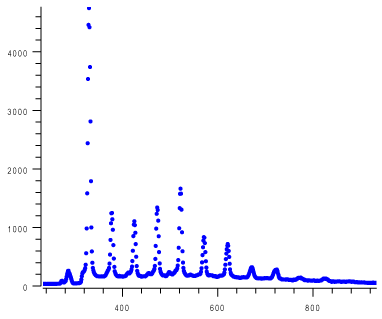
\includegraphics[width=0.45\textwidth]{AgBeh_sdist_22}
	\caption[Diffraction from AgBeh on glass cover slip at \motor\ = 22\dg\ or $\omega$ = 5\dg and $q_z$ plot along the meridian]{Diffraction from AgBeh on glass cover slip at \motor\ = 22\dg\ or $\omega$ = 5\dg and $q_z$ plot along the meridian. The peak positions are fitted in the ds program to calculate the s-distance assuming the D-spacing of AgBeh is 58.367 \AA. The calculated s-distance is 123.29 mm.}
	\label{fig:AgBeh22deg}
\end{figure}
%------------------------------------------------------------------
Note, however, that the shapes of the peaks are somewhat distorted at a fixed angle compared to those when a sample is rotated. (Why???) This increases the error in measuring the distance. In order to characterize this point, the s-distance was measured with the usual rotation method in the LAXS setup, and then D-spacings were measured at various fixed angles with the same setup [See Table \ref{tab:AgBehComparison}].
%------------------------------------------------------------------
\begin{figure}[htbp]
	\centering
	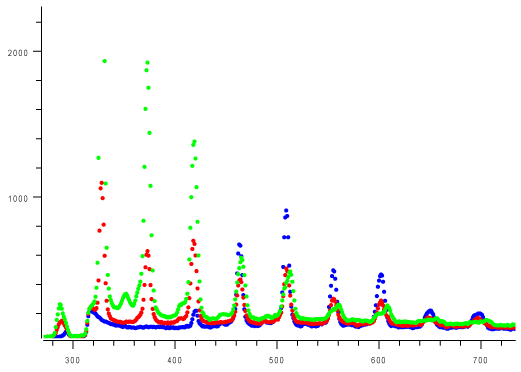
\includegraphics[width=\textwidth]{AgBehComparison}
	\caption[Comparison of shapes of the peaks]{Comparison of shapes of the peaks. (red) rotation, (green) \motor\ = 1\dg, and (blue) \motor\ = 5\dg. The sample is AgBeh on a silicon wafer in the LAXS experimental setup.}
	\label{fig:AgBehComparison}
\end{figure}
%------------------------------------------------------------------
\begin{table}[htbp]
	\centering
	\subfloat{
	\begin{tabular}{c|cc}
			\hline		
			$\omega$	& $D$	(\AA)	& peaks fitted	\\ \hline
						&		& 	\\
			1\dg 	& 57.92   & 1-7th		\\
			2\dg 	& 58.14 	& 2-9th		\\
			3\dg  & 57.99 	& 3-9th 	\\
			4\dg  & 58.40   & 3-9th  	\\
			5\dg 	& 58.37 	& 4-9th  	\\
			6\dg	& 58.28 	& 5-11th 	\\
			7\dg	& 58.32   & 5-10th	\\
			\hline
	\end{tabular}}
	\qquad
	\subfloat{
	\begin{tabular}{c|cc}
			\hline		
			$\omega$	& $S$	(mm)	& peaks fitted	\\ \hline
			rot		&	116.14	& 	\\
			1\dg 	& 117.27   & 1-7th		\\
			2\dg 	& 116.69 	& 2-9th		\\
			3\dg  & 116.80 	& 3-9th 	\\
			4\dg  & 116.26   & 3-9th  	\\
			5\dg 	& 116.22 	& 4-9th  	\\
			6\dg	& 116.35 	& 5-11th 	\\
			7\dg	& 116.36   & 5-10th	\\
			\hline
	\end{tabular}}
	\caption[Tables of apparent D-spacings of AgBeh and measured S-distance at various fixed angles]{Tables of apparent D-spacings of AgBeh and measured S-distance at various fixed angles. Apparent D-spacings are determined using $S$ = 116.14 mm. The substrate is the usual silicon wafer. The sample holder is the one for LAXS experiments. Files: sc\_0360.img - sc\_0367.img.}
	\label{tab:AgBehComparison}
\end{table}
%-----------------------------------------------------------------

From Figure \ref{fig:sgeometry}, S-distance at any \motor\ is given by
\begin{align}
	S(\theta_m) &= S(22^{\circ}) - \Delta S \nonumber\\
							&= S(22^{\circ}) - R(\sin 22^{\circ} - \sin\theta_m),
\end{align}
where the radius, $R$ is equal to 21.10 mm and $S(22^{\circ})$ = 123.29 mm. \motor\ is positive at glancing angles and negative at the transmission angle. For the transmission angle, \motor\ = $-28$\dg, and S-distance is calculated to be 105.48 mm.
%------------------------------------------------------------------
\begin{figure}[htbp]
	\centering
	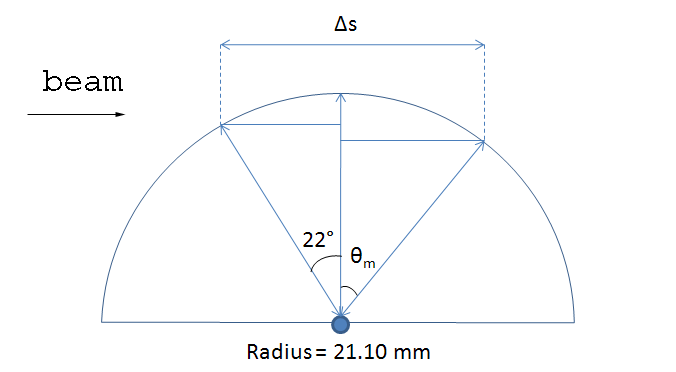
\includegraphics[width=0.5\textwidth]{sgeometry}
	\caption[A diagram showing how $\Delta s$, the distance between the sample position at \motor\ = 22\dg\ and an arbitrary \motor, is calculated]{A diagram showing how $\Delta s$, the distance between the sample position at \motor\ = 22\dg\ and an arbitrary \motor, is calculated. \motor\ has a negative value in this geometry.}
	\label{fig:sgeometry}
\end{figure}
%------------------------------------------------------------------
\begin{figure}[htbp]
	\centering
	\subfloat[][On glass cover slip. $\omega$ = 45\dg.]{
		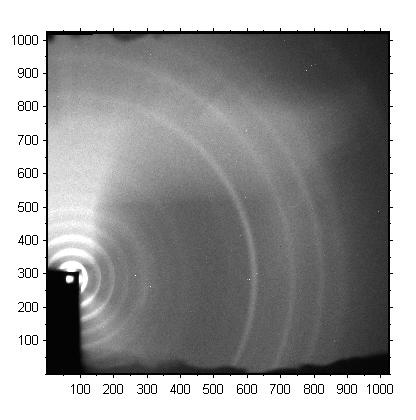
\includegraphics[width=0.4\textwidth]{AgBeh_n28}
		\label{fig:AgBeh28}}
	\qquad
%	\subfloat[][On silicon wafer. The sample is rotated during exposure.]{
%		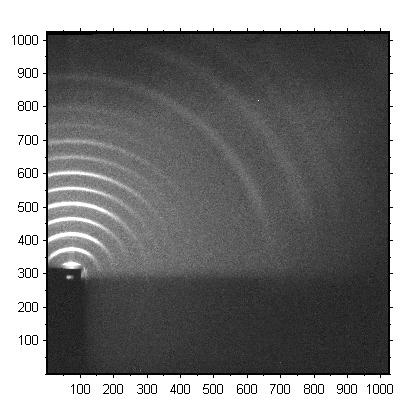
\includegraphics[width=0.3\textwidth]{AgBeh_rot}
%		\label{fig:AgBehRot}}
%	\qquad
	\subfloat[][On silicon wafer. \motor\ = $\omega=5$\dg.]{
		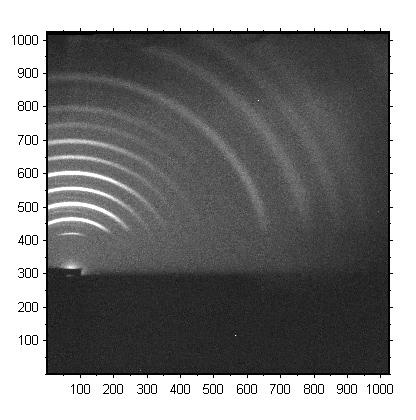
\includegraphics[width=0.4\textwidth]{AgBeh_5}
		\label{fig:AgBeh5}}
	\caption[Diffraction from AgBeh on different substrates]{Diffraction from AgBeh on different substrates. (a) Glass coverslip is on WAXS holder. (b) Silicon wafer is on LAXS holder. For (a), a piece of lead tape was not attached to the back of the sample holder [as described in the Overview of the Experiment section]; therefore, a light region is seen in (a) between $p_z$ = 500 and 800.  Because the silicon wafer is very thick compared to the glass cover slip, scattering is strongly blocked below $p_z$ = 400 in (b) whereas scattering is only partially blocked in Figure \ref{fig:AgBeh22deg}. Both images are taken with the same CCD position.}
\end{figure}
%------------------------------------------------------------------
\newpage
\section{Background Scattering}
The substrate used in the transmission experiments is a glass coverslip with thickness $75\,\mathrm{\mu m}$. It is an amorphous material and gives rise to diffuse scattering when exposed to an x-ray beam. Figure \ref{fig:Background} shows scattering with and without a glass coverslip at $\omega=45$\dg before and after helium is put into the chamber. Note the bright halo in regions that are about 600 pixels away from the direct beam when a glass coverslip is present. The region with high intensity above the direct beam seen in all four pictures is due to air scattering in R0, which is present whether or not helium is used in the chamber. 
\begin{figure}[htbp]
	\centering
	\subfloat[][No substrate without He (NSWOHe). {[0 2400]} ]{	
		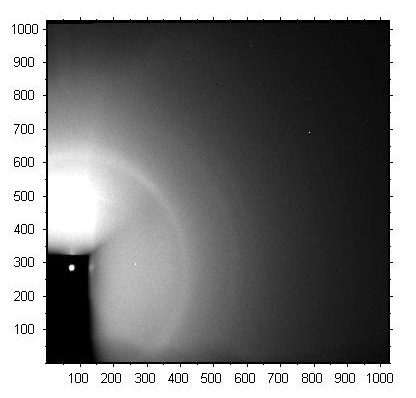
\includegraphics[width=0.4\textwidth]{noGlass_t}}
	\qquad
	\subfloat[][No substrate with He (NSWHe). {[0 800]}]{
		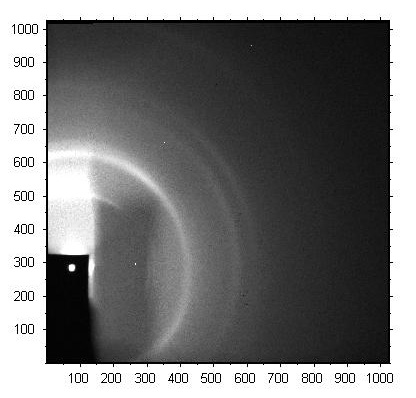
\includegraphics[width=0.4\textwidth]{noGlass_t_he}}
	\qquad
	\subfloat[][Glass without He (GWOHe). {[0 1200]}]{
		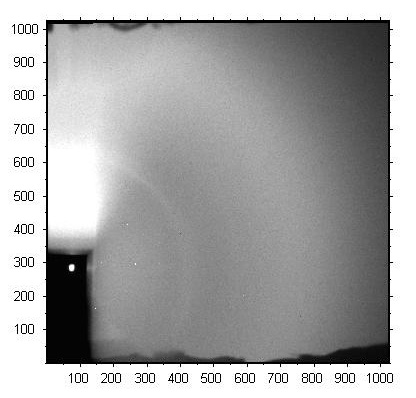
\includegraphics[width=0.4\textwidth]{glass_t}}
	\qquad
	\subfloat[][Glass with He (GWHe). {[0 1200]}]{
		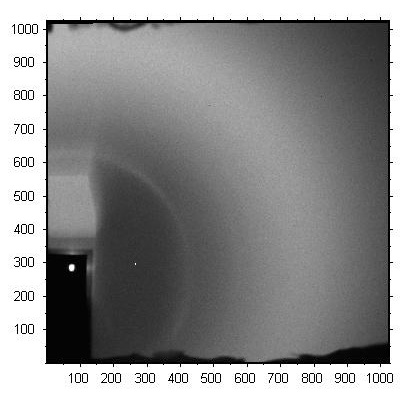
\includegraphics[width=0.4\textwidth]{glass_t_he}}
	\caption[Scattering from a glass cover slip or no substrate, with and without helium (He)]{Scattering from a glass cover slip or no substrate, with and without helium (He). $s$ = 105.48 mm.} %raw data files: (a) rt_0219.img, (b) rt_0210.img, (c) sc_0536.img, (d) sc_0535.img.
	\label{fig:Background}
\end{figure}

Figure \ref{fig:GlassQrplot} is a $p_x$ plot centered at $p_z$ = 286 $\pm$ 10 pixels. A sharp peak appearing at $p_x\approx 80$ is the attenuated beam. Comparison between the plots of glass with helium (GWHe/Blue) and no substrate with helium (NSWHe/Green) shows the scattering due to a glass cover slip. It has strong diffuse scattering, peaked around $p_x=750$, which is where WAXS peaks from the gel and ripple phases appear as we shall see later. Comparison between glass with and without helium tells us that photons scattered by air do not reach over $p_x=800$. An interesting feature is no substrate without helium (NSWOHe/Red) scatters stronger below $p_x=600$ (crossover between cyan and red) than glass without helium (GWOHe/Cyan) does. This is somewhat counter-intuitive because both have the same density of air but one with an extra scattering object, the glass. An important point to note here is that the substrate absorbs the beam and cuts down the intensity by approximately 60\%. Therefore, the strong intensity of NSWOHe/Red between $p_x=150$ and 450 is due to air in region R3 and R4. Also note that between $p_x=300$ and 450, NSWHe/Green has some extra scattering that GWHe/Blue does not. This may be the diffuse scattering from Mylar exit windows. The intensity of NSWHe/Green seems to get cut down by something at $p_x=300$. This is perhaps due to the beam stop. (These statements need to be confirmed.)

Figure \ref{fig:GlassQzplot} is a $p_z$ plot centered at $p_x=71$ $\pm$ 10 pixels. The point at which the cyan and blue curves cross is approximately $p_z=980$, or $980-286$ = 694 pixels from the beam center. In Figure \ref{fig:GlassQrplot}, the peak of the blue curve is seen to be located at $p_x=750$, or $750-71$ = 679 pixels from the beam center. Thus, the diffuse scattering from a glass cover slip is isotropic, which is clear from Figure \ref{fig:Background}(d). 
	In conclusion, a glass coverslip gives diffuse scattering that is especially intense at $\sqrt{\mathrm{x}^2+\mathrm{y}^2}\approx 690$ pixels or $q \approx 1.7$ \iang, which is particularly important in WAXS experiments. 

%-------------------------------------------------------------
\begin{figure}[htbp]
	\centering
	\subfloat[][$p_x$ plot along the horizon]{
		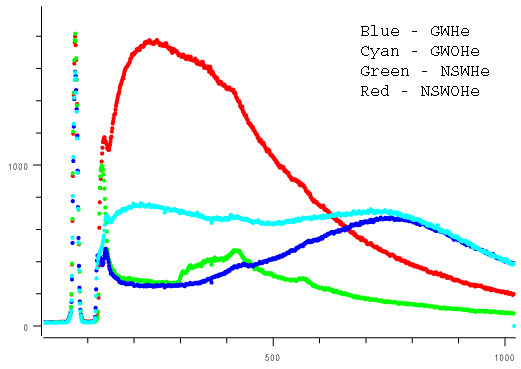
\includegraphics[width=0.5\textwidth]{GlassScatteringQrplot1}
		\label{fig:GlassQrplot}}
	\subfloat[][$p_z$ plot along the meridian]{	
		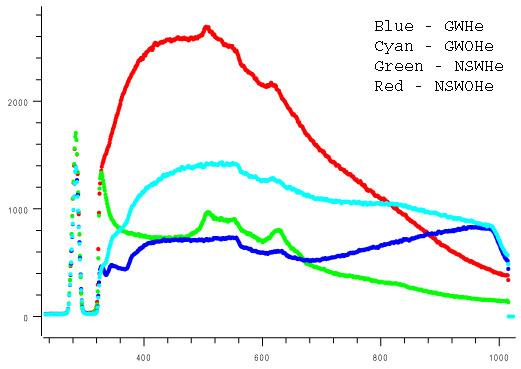
\includegraphics[width=0.5\textwidth]{GlassScatteringQzplot1}
		\label{fig:GlassQzplot}}
	\caption[$p_x$ and $p_z$ plots of intensity from a glasscover slip or no substrate]{$p_x$ and $p_z$ plots of intensity from a glass coverslip or no substrate. (Blue) GWHe, (cyan) GWOHe, (green) NSWHe, and (red) NSWOHe.}
\end{figure}
%---------------------------------------------------------------
\newpage
\section{Geometric Broadening}
Assume that the beam has a rectangular cross section with its height $Y_b$ and width $X_b$ and is parallel to the lab y axis as shown in Figure \ref{fig:TransmissionGeometry}. When the sample is tilted by $\omega$ with respect to the lab x-y plane as in transmission experiments, rays emerging from the top edge of the sample travel extra distance compared to the distance that rays from the bottom edge of the sample travel. This, then, leads to distortion of the scattered beam; namely, the scattered beam will appear on the CCD screen as a parallelogram as shown in Figure \ref{fig:GeometricBroadening1}. Figure \ref{fig:GeometricBroadening2} shows the top- and sideview of the projection of the beam on the sample. From simple geometry, it can be shown that $a=Y_b/\tan\omega$, $b=aX/(2S)$, $c=aZ/(2S)+Y_B/2$, and $B=\tan^{-1}(Z/S)$. Since $H=2c$ and $W=2b$, $H$ and $W$ in Figure \ref{fig:parallelogram} are given by
\begin{align}
	H &= Y_b\left(1+\frac{Z}{S\tan\omega}\right)\\
	W &= Y_b\frac{X}{S\tan\omega}.
\end{align}
The parallelogram in Figure \ref{fig:parallelogram} illustrates the geometric broadening of a delta function peak on the CCD detector in transmission experiments. 
\begin{figure}[htbp]
	\centering
	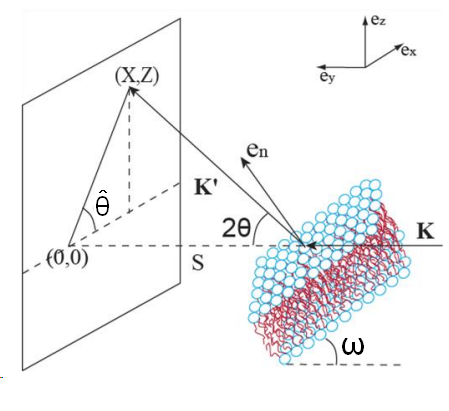
\includegraphics[width=0.5\textwidth]{TransmissionGeometry}
	\caption[The transmission experiment geometry]{The transmission experiment geometry. $\mathbf{k}$ is the wave vector of the incident beam; $\mathbf{k^{'}}$ is the wave vector of the scattered beam; $2\theta$ is the angle between the scattered and incident beam commonly referred to as the Bragg scattering angle; $\omega$ is the tilt angle of the sample about the x axis relative to the x-y plane;  $\mathbf{e_n}$ is the unit vector along the sample normal; the beam position is taken to be the origin for simplicity in the CCD frame; ($X$,$Z$) is the position of the scattered beam on the CCD detector; $\hat{\theta}$ is the angle between ($X$,$Z$) and the +X axis; $s$ is the distance between the sample and the detector.}
	\label{fig:TransmissionGeometry}
\end{figure}
\begin{figure}
	\centering
	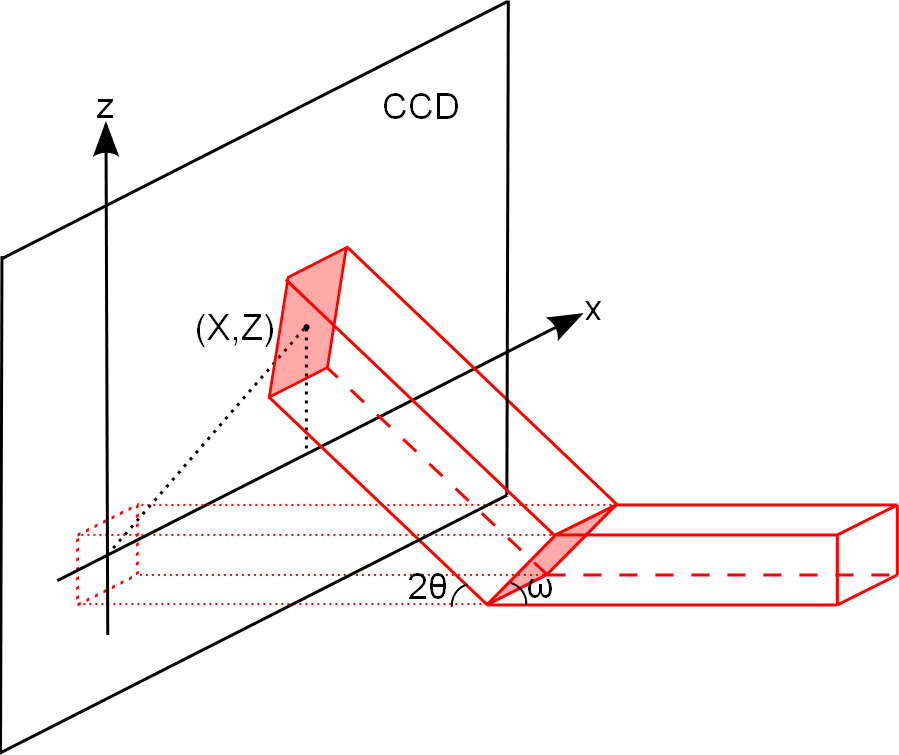
\includegraphics[width=0.5\textwidth]{GeometricBroadening1}
	\caption{A diagram showing how the beam is scattered. The projection of the beam on the sample and of the scattered beam on the detector are shaded. The sample is tilted by $\omega$ with respect to the lab x-y plane. The lab y-axis is in the direction of the incoming beam. The red dots show the transmitted beam. The beam is rectangular but upon scattering with total Bragg angle $2\theta$ appears as a parallelogram on the CCD. Note that the lab x- and z- axis are drawn such that a rectangle looks like a parallelogram in this diagram.}
	\label{fig:GeometricBroadening1}
\end{figure}
\begin{figure}
	\centering
	\subfloat[Topview]{
		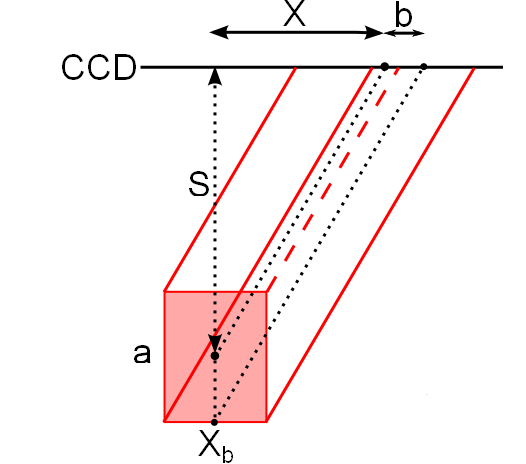
\includegraphics[width=0.5\textwidth]{GeometricBroadening2}}
%	\qquad
	\subfloat[Sideview]{
		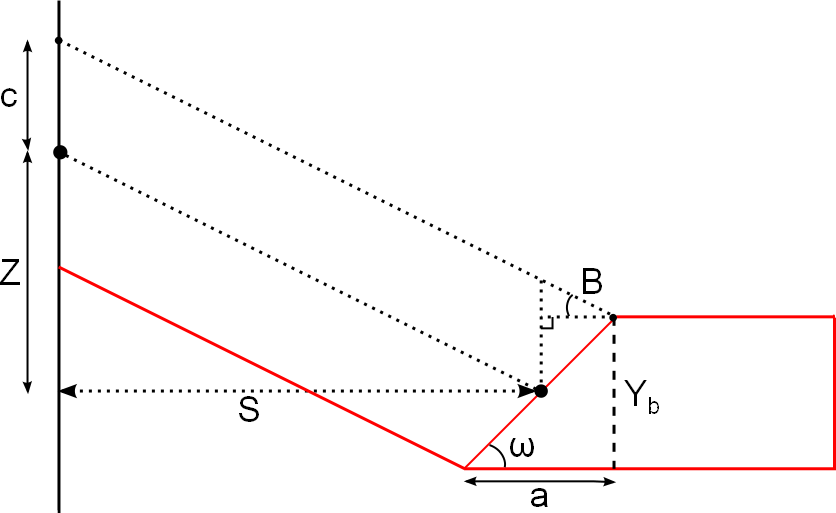
\includegraphics[width=0.5\textwidth]{GeometricBroadening3}}
	\caption{Topview and sideview of the projection of the beam on the sample tilted at $\omega$ with respect to the lab x-y plane. The formula for lengths a, b, and c and angle B are shown in the text. $X_b$ is the beam width and $Y_b$ the beam height. $S$ is the S-distance. $(X,Z)$ is a position of the center of the scattered beam on the detector with respect to the center of the transmitted beam as shown in Figure \ref{fig:GeometricBroadening1}. The black dotted lines in (b) correspond to those in (a). The red rays coming from the top of the sample are not shown in (b).}
	\label{fig:GeometricBroadening2}
\end{figure}
\begin{figure}[htbp]
	\centering
	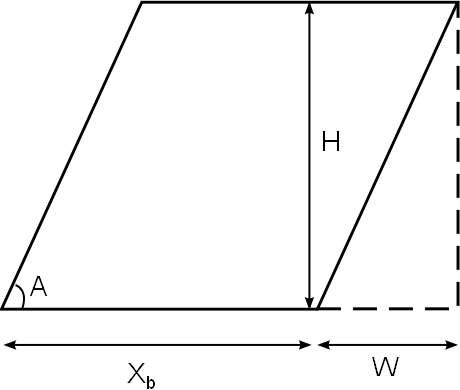
\includegraphics[width = 0.3\textwidth]{GeometricBroadening4}
	\caption{A scattered beam appears as a parallelogram on the CCD detector.}
	\label{fig:parallelogram}
\end{figure}
%----------------------------------------------------------------------
\newpage
\section{D-spacing}
The D-spacing of the DMPC sample is measured in a similar way as the s-distance. To determin the D-spacing, however, the s-distance measured earlier is input into the ds program. $s$ = 123.29 mm was obtained at $\omega$ = 5\dg\ using a AgBeh sample. Then, at $\omega$ = 3\dg, $s$ was calculated to be 122.60 mm. (I should have measured s-distance at 20\dg\ instead.)
%---------------------------------------------------------------
\begin{figure}[htbp]
	\centering
	\subfloat[][$\omega$ = 3\dg. $s$ = 122.60 mm.]{
		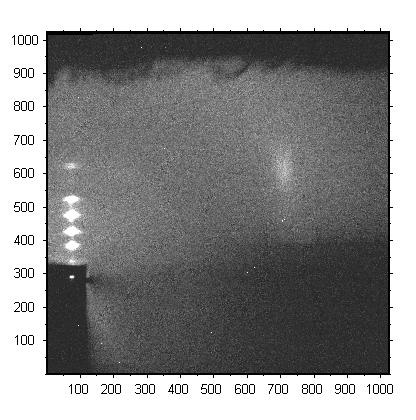
\includegraphics[width=0.4\textwidth]{gel_g52_20}
		\label{fig:GelDspace1}}
	\qquad
	\subfloat[][$\omega$ = 3\dg. $q_z$ plot along the meridian. 2, 3, 4, 5, and 7th peaks were fitted.]{
		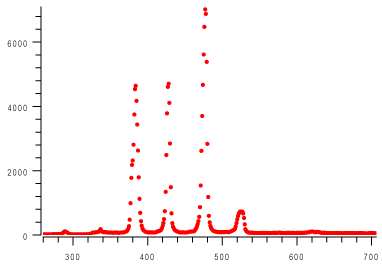
\includegraphics[width=0.4\textwidth]{gel_laxs_qzplot1}
		\label{fig:GelDspace2}}
	\qquad
	\subfloat[][$\omega$ = 5\dg. $s$ = 123.29 mm.]{
		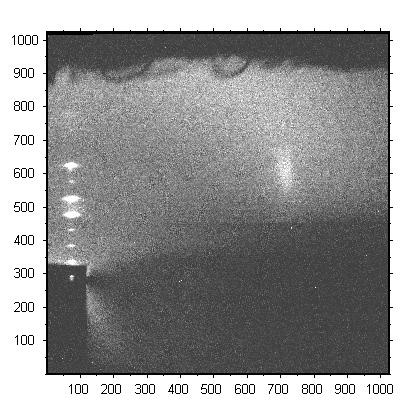
\includegraphics[width=0.4\textwidth]{gel_g52_22}
		\label{fig:GelDspace3}}
	\qquad
	\subfloat[][$\omega$ = 5\dg. $q_z$ plot along the meridian. 4, 5, and 7th peaks were fitted.]{
		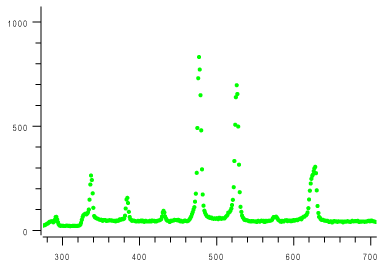
\includegraphics[width=0.4\textwidth]{gel_laxs_qzplot2}
		\label{fig:GelDspace4}}
	\caption[gel phase DMPC at fixed glancing angles]{gel phase DMPC at fixed glancing angles. $D$ = 57.91 \AA\ and 57.95 \AA\ at $\omega$ = 3\dg\ and 5\dg, respectively.}	
\end{figure}
%---------------------------------------------------------------
\newpage
\section{Light Background Subtraction}
The diffuse scattering from a glass substrate necessitates what is called light background subtraction. To obtain a light background, a glass cover slip with no lipids is placed on the sample holder and exposed for twenty minutes with dezingering.
%---------------------------------------------------------------
\begin{figure}[htbp]
	\centering
	\subfloat[gel phase DMPC at $\omega=45$\dg][Scattering from oriented bilayers of gel phase DMPC taken at $\omega=45$\dg. Four 2x1200s (20 minutes, dezingered) images are added together for a better signal-to-noise ratio.]{
		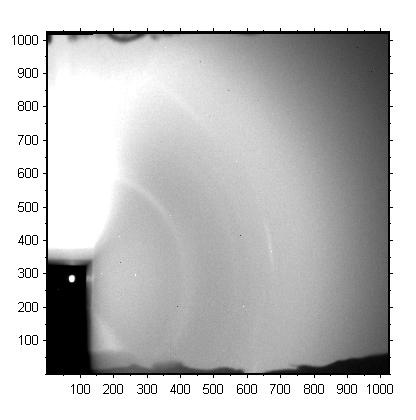
\includegraphics[width=0.44\linewidth]{gel_t52_smpl}
		\label{fig:GelSample}}
	\qquad
	\subfloat[Light background][Scattering from the substrate taken at $\omega=45$\dg, called light background. Four 2x1200s images are added together.]{
	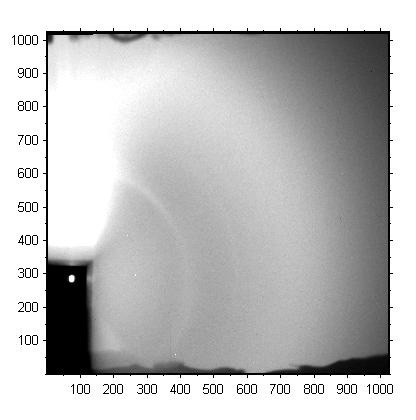
\includegraphics[width=0.44\linewidth]{gel_t52_bkgnd}
	\label{fig:GelBackground}}
	\caption{Sample and Light background}
\end{figure}
%------------------------
\begin{figure}[htbp]
	\centering
	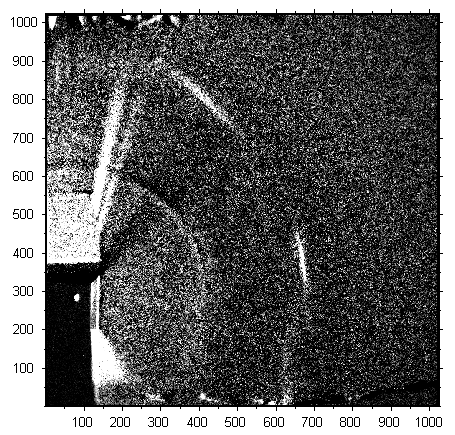
\includegraphics[width=0.6\textwidth]{gel_t52}
	\caption[gel phase DMPC after light background subtraction]{An image obtained by subtracting data shown in Figure \ref{fig:GelBackground} (background) from data in Figure \ref{fig:GelSample} (sample). [0 150]}
	\label{fig:GelCCD}
\end{figure}
%-----------------------------------------------------------------

\newpage
\section{Transformation from CCD- to q-space}
Because a sample is tilted by 45\dg with respect to the lab xy plane, y and z axes in the sample q-space do not coincide with those of the lab coordinates. In order to obtain a scattering intensity map in  sample q-space, an appropriate transformation must be applied to a picture directly obtained from the CCD screen. Figure \ref{fig:GelTrans} is the diffraction pattern from gel phase DMPC in q-space obtained after such transformation is applied to Figure \ref{fig:GelCCD}. Details are discussed in Jianjun Pan$'$s thesis, chapter 5.3. The transformation is applied using MATLAB. 
%------------------------------------------------------------------
\begin{figure}[htbp]
	\centering
	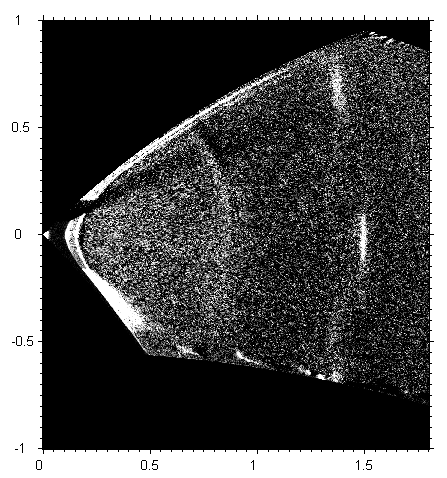
\includegraphics[width=0.6\textwidth]{gel_t52_trans}
	\caption[Gel phase pattern in q-space]{An image obtained after transforming data in Figure \ref{fig:GelCCD} into q-space. The horizontal axis is $q_r$ and vertical $q_z$ in units of \AA$^{-1}$. [0 150]}
	\label{fig:GelTrans}
\end{figure}

%------------------------------------------------------------------
\newpage
\section{Transmission experiment at 10 \dg C: the gel phase}
In this section, gel phase experiments are discussed. Gel phase experiments are completed to make sure that the sample scatters as expected and assess the sample$'$s quality. Since the ripple phase is hypothesized to have a gel phase like packing in the major side, gel phase pictures will give an idea of what to expect in the ripple phase. Another advantage is that it will demonstrate if the CCD screen is rotated about the beam axis with respect to the lab coordinates. In other words, if the sample $q_z$ axis is parallel to the lab z-axis, then the (20) peak will appear at $q_z$ = 0 after a picture in CCD-space is transformed into q-space.
%---------------------------------------------------------------
\begin{figure}[htbp]
	\centering
	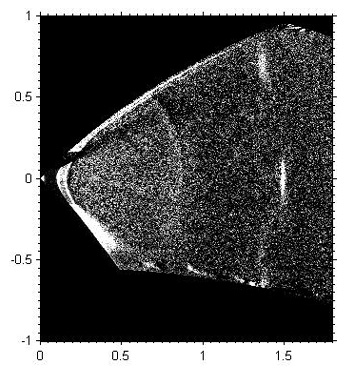
\includegraphics[width=0.4\textwidth]{gel_t52_rot_trans}
	\caption[Intensity map of gel phase in q-space with 1\dg\ rotation]{Gel phase DMPC with 1\dg\ counter-clockwise rotation applied prior to the transformation.}
%(a) File name: “gel_t52_trans.fig”
%(b) File name: “gel_t52_trans_rot.fig”
	\label{fig:GelTransRot}
\end{figure}
%---------------------------------------------------------------

Figure \ref{fig:GelTrans} shows scattering intensity maps in the gel phase in q-space, taken at angle of incidence of 45\dg. Figure \ref{fig:GelTransRot} shows diffraction from the gel phase when Figure \ref{fig:GelCCD} is rotated by 1\dg\ counter-clockwise before it is transformed into q-space. 

Figure \ref{fig:GelQr} and \ref{fig:GelQz} show $q_r$- and $q_z$-plots of the (20) peak fitted with a Gaussian, respectively. The fitting function is given by
\begin{equation}
	y=y_0 + \frac{A}{w \sqrt{\pi /2}}\,\mathrm{exp}\left[ -2\left(\frac{(x-x_c)}{w}\right)^2\right].
\end{equation}	

Table \ref{tab:GaussianQr} and \ref{tab:GaussianQz} list values for fitted parameters in rotated and non-rotated cases in the $q_r$ and $q_z$ direction, respectively. The peak position in $q_r$ is approximately equal to 1.49 \iang.
%-----------q_r plots of (20) peak of the gel phase------------
\begin{figure}[htbp]
	\centering
	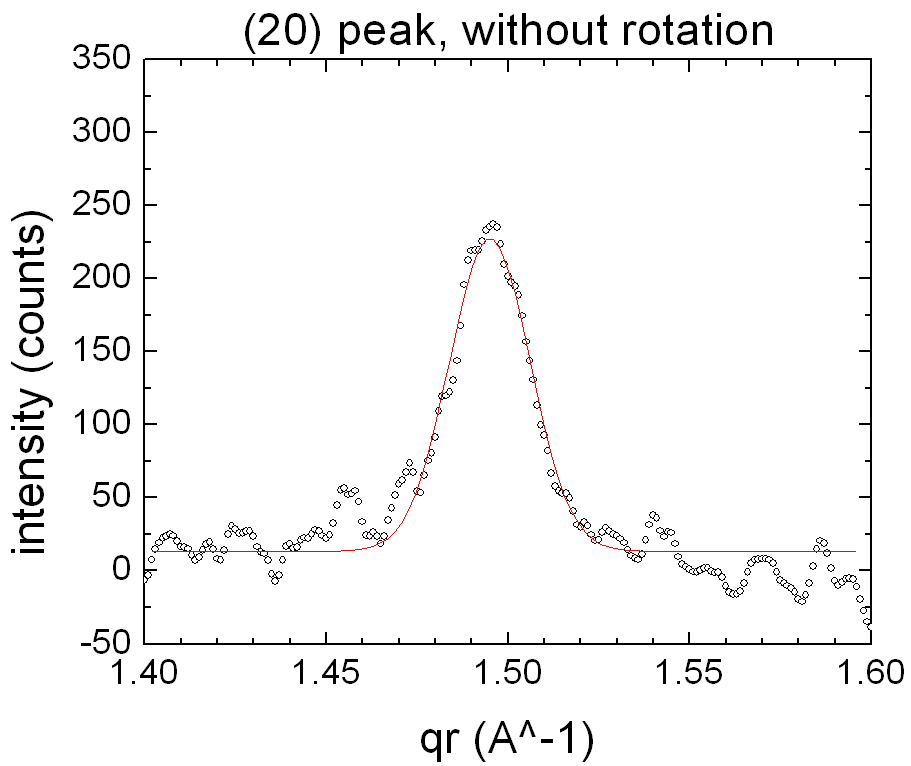
\includegraphics[width=0.45\textwidth]{gel_20peak_qrplot1}
	\qquad
	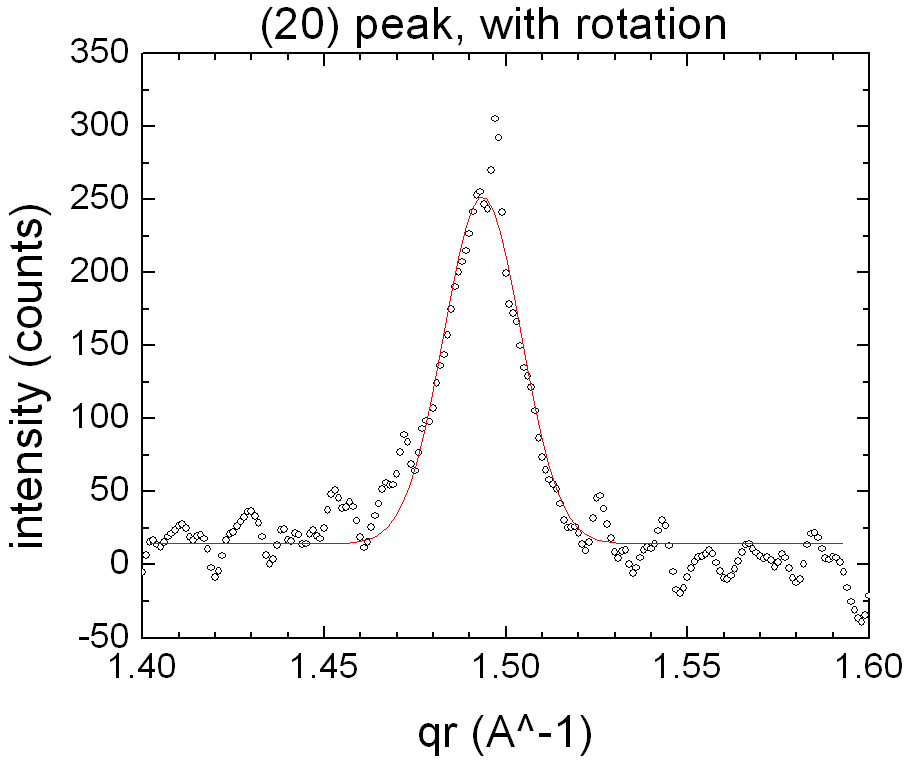
\includegraphics[width=0.45\textwidth]{gel_20peak_qrplot2}
	\caption[$q_r$ plots of (20) peak of the gel phase]{$q_r$ plots of (20) peak of the gel phase centered at $q_z = 0$ \iang\ averaged for $\pm 0.040$ \iang\ with and without 1\dg\ rotation applied counter-clockwise prior to the transformation. The solid red curve is a Gaussian fit.} 
	\label{fig:GelQr}
\end{figure}
%-----------------Fitted parameters in q_r----------------------
\begin{table}[htbp]
	\centering
	\subfloat[][Non-rotated]{
		\begin{tabular}{c|cc}
			      	& Value		& Standard	\\
			      	&					& Error		\\ \hline
			$y_0$ 	& 13.45   & 1.308		\\
			$x_c$ 	& 1.495   & 2.516E-4	\\
			$w$   	& 0.02218 & 5.383E-4 	\\
			$A$   	& 5.961   & 0.1402   	\\
			sigma 	& 0.01109 &          	\\
			FWHM		& 0.02611 &         	\\
			Height	& 214.5   &   		\\
		\end{tabular}
		\label{tab:GaussianQr1}}
	\qquad
	\subfloat[][Rotated by 1\dg\ CCW]{
		\begin{tabular}{c|cc}	
			      	& Value		& Standard	\\
			      	&					& Error		\\ \hline
			$y_0$ 	& 14.43   & 1.404		\\
			$x_c$ 	& 1.494   & 2.380E-4	\\
			$w$   	& 0.02124 & 5.080E-4 	\\
			$A$   	& 6.328   & 0.1462   	\\
			sigma 	& 0.01062 &          	\\
			FWHM		& 0.02501 &         	\\
			Height	& 237.7   &   		\\
		\end{tabular}
		\label{tab:GaussianQr2}}
	\caption{Values of fitted parameters in $q_r$ direction.}
	\label{tab:GaussianQr}
\end{table}
%-------------q_z plots of (20) peak of gel phase----------------
\begin{figure}[htbp]
	\centering
	\begin{minipage}[b]{0.45\linewidth}
		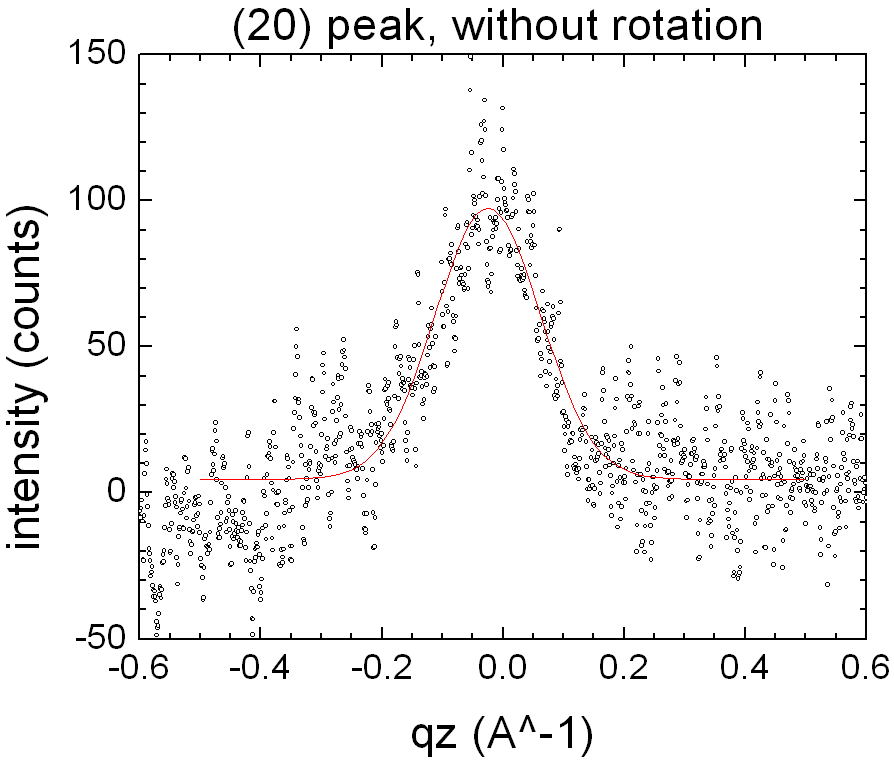
\includegraphics[width=\linewidth]{gel_20peak_qzplot1}
	\end{minipage}
	\qquad
	\begin{minipage}[b]{0.45\linewidth}
		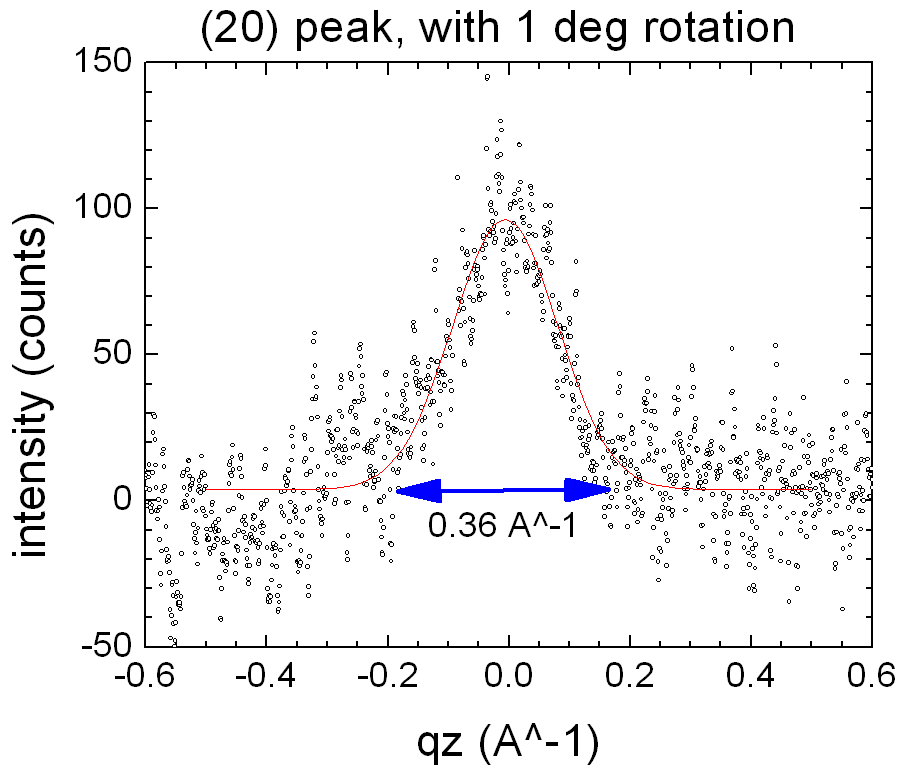
\includegraphics[width=\linewidth]{gel_20peak_qzplot2}
	\end{minipage}
	\caption[$q_z$ plots of (20) peak of the gel phase]{$q_z$ plots of (20) peak of the gel phase centered at $q_r = 1.495$ \iang averaged for $\pm 0.040$ \iang\ with and without 1\dg\ rotation applied counter-clockwise prior to the transformation. The solid red curve is a Gaussian fit.}
%File name: “gel_20peak_qzplot1.png”
%File name: “gel_20peak_qzplot2.png” 
	\label{fig:GelQz}
\end{figure}
%-----------------Fitted parameters in q_z-------------------
\begin{table}[htbp]
	\centering
	\subfloat[][Non-rotated]{
		\begin{tabular}{c|cc}
			\hline		
			      	& Value		& Standard	\\
			      	&					& Error		\\ \hline
			$y_0$ 	& 4.646   & 0.766		\\
			$x_c$ 	& -0.025 	& 0.002	\\
			$w$   	& 0.1741 	& 0.0043 	\\
			$A$   	& 20.26   & 0.53  	\\
			sigma 	& 0.08703 &          	\\
			FWHM		& 0.2049 	&         	\\
			Height	& 92.87   &   		\\
			\hline
		\end{tabular}
		\label{tab:GaussianQz1}}
	\qquad
	\subfloat[][Rotated by 1\dg\ CCW]{
		\begin{tabular}{c|cc}
			\hline		
			      	& Value		& Standard	\\
			      	&					& Error		\\ \hline
			$y_0$ 	& 3.884   & 0.762	\\
			$x_c$ 	& -0.006  & 0.002	\\
			$w$   	& 0.1745 	& 0.0043	\\
			$A$   	& 20.21  	& 0.52 	\\
			sigma 	& 0.08723 &          	\\
			FWHM		& 0.2054 	&         	\\
			Height	& 92.41  	&   		\\
			\hline
		\end{tabular}
		\label{tab:GaussianQz2}}
	\caption{Values of fitted parameters in the $q_z$ direction.}
	\label{tab:GaussianQz}
\end{table}
%----------------------------------------------------------------

Figure \ref{fig:Gel20peakCCDqr} is a plot in the horizontal direction of (20) peak averaged from y = 390 to 410 in CCD-space. [See Figure \ref{fig:GelCCD}] From the plot, the width of the peak is found to be approximately 10 pixels, or 0.68 mm. This is almost equal to the width of the beam itself. Hence, broadening of the peak is attributed to geometric broadening. In fact, the intrinsic width of this peak was previously found to be much smaller than what can be probed in the current setup. The corresponding broadening in q-space is 0.025 \iang, which is the value of FWHM found in Table \ref{tab:GaussianQr2}.
\begin{figure}[htbp]
	\centering
	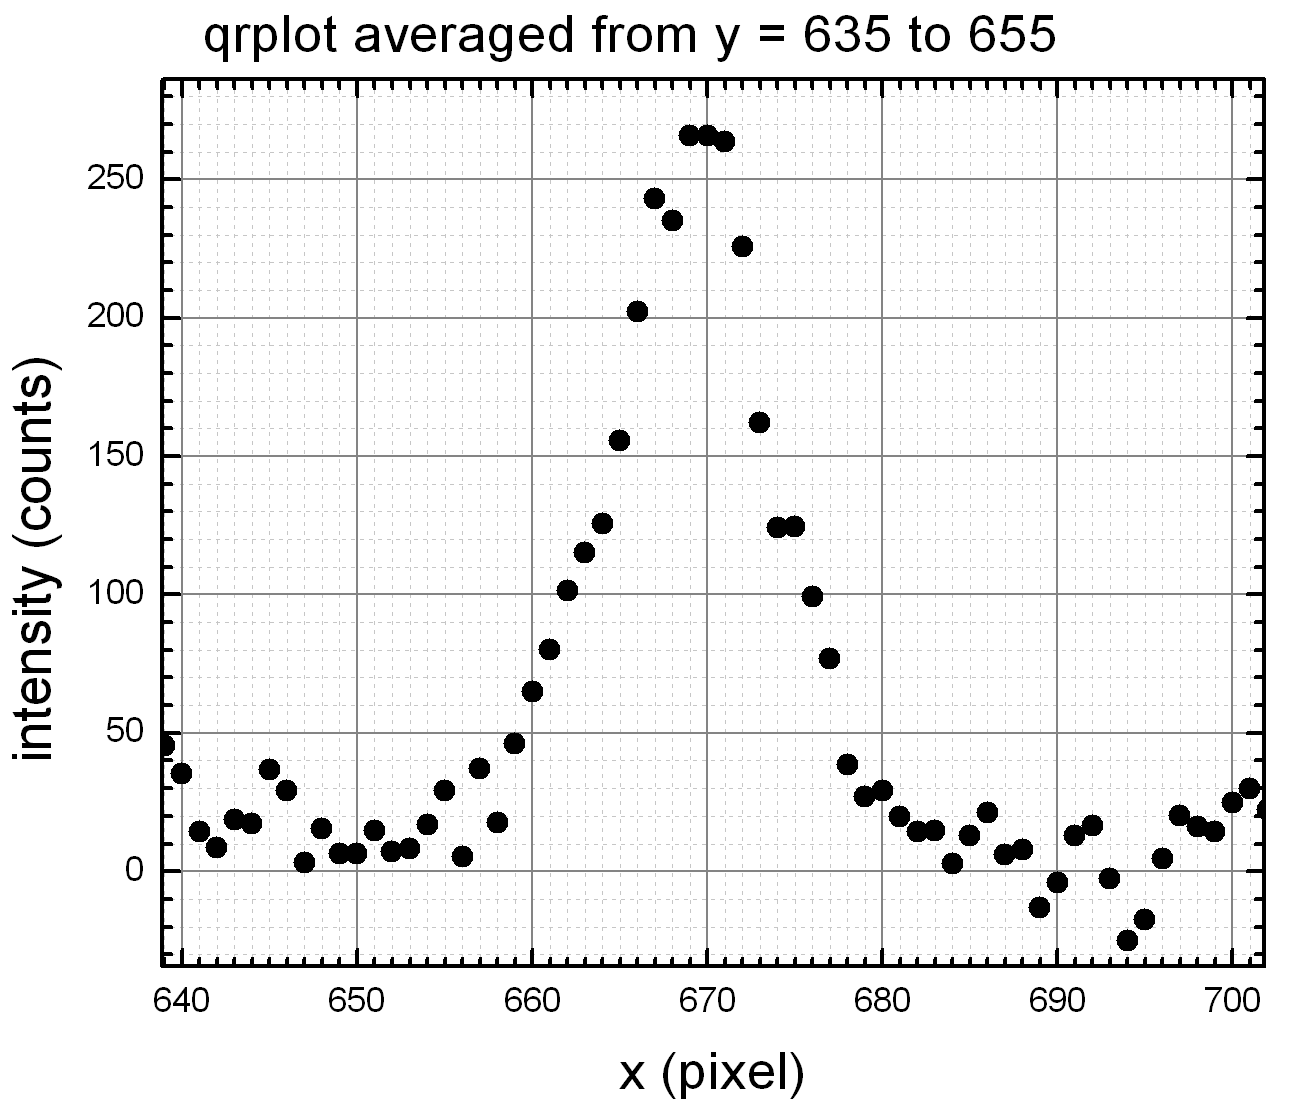
\includegraphics[width=0.5\textwidth]{gel20qr}
	\caption[A plot in the horizontal direction of (20) peak]{A plot in the horizontal direction of (20) peak. Centered at y = 400 and averaged from y = 390 to 410.}
	\label{fig:Gel20peakCCDqr}
\end{figure}

The peak position in the $q_z$ direction is given by the values of $x_c$. Note that after 1\dg\ rotation CCW, the $x_c$ got closer to 0 \iang.  When rotated by 2\dg\ CCW, $x_c$ became positive. [Data not shown] Hence, the true rotation angle for correction of the CCD screen is between 1\dg\ and 2\dg. Originally, a ripple phase picture was planned to be used along with a gel phase one to confirm the rotation angle. However, the obtained ripple phase data was very noisy, which made it difficult to measure the exact positions of the peaks above and below the equator. A less noisy picture of the gel phase is also desired to increase the accuracy of this method. (What is the signal to noise ratio currently?)

(Maybe I should put this analysis in a separate section?) In the thin rod model, which will be discussed in the Thin Rod Model of the ripple phase section, the intensity of a Bragg rod is proportional to 
\begin{equation}
	\left[\frac{4}{\gamma}\sin \left(\frac{L\gamma}{2}\right)\right]^2,
\end{equation}
where $\gamma=\alpha q_x+\beta q_y +q_z$, $\alpha=\tan\theta_t\cos\phi$, and $\beta=\tan\theta_t\sin\phi$. In $L_{\beta I}$ phase, where (20) peak appears on the equator, $\phi=90$\dg. Since $q_y=0$ for the (20) peak according to the Laue condition, then, $\gamma = q_z$, which gives the full width of the peak, $\Delta q_z$, equal to $4\pi/L$, where L is the length of a rod. From Figure \ref{fig:GelQz}, $\Delta q_z$ is estimated to be 0.36 \iang, which yields L = 34.9 \AA. It is known that this value should be either approximately 20 or 40 \AA, depending on whether two chains scatter coherently or only one chain does. From Figure \ref{fig:GelQz}, L clearly cannot be 20 \AA. Hence, it is likely that two chains scatter coherently.

%----------------------------------------------------------------
\newpage
\section{Transmission experiment at 18 \dg C: the ripple phase}
Figure \ref{fig:RippleCCDRot} shows a diffraction pattern from DMPC in the ripple phase at 18 \dg C with 1\dg\ CCW rotation applied. Figure \ref{fig:RippleTransRot} is the corresponding image in q-space. The sample is slightly dehydrated by a heating Peltier, which gives approximately $D$ = 58.2 \AA.
%-----------------ripple phase images----------------------------
\begin{figure}[htbp]
	\centering
	\includegraphics[width=0.5\textwidth]{ripple_t52_rot}
	\caption[Diffraction from ripple phase DMPC in CCD-space]{Diffraction from ripple phase DMPC in CCD-space. T = 18 \dg C. 1\dg\ CCW rotation applied. A bright region around (x,y)=(200,100) and less bright region above the beam are both due to imperfect light background subtraction. [0 150]}
	\label{fig:RippleCCDRot}
\end{figure}
\begin{figure}[htbp]
	\centering
	\includegraphics[width=0.5\textwidth]{ripple_t52_rot_trans}
	\caption[Diffraction from ripple phase DMPC in q-space]{Diffraction from ripple phase DMPC in q-space, corresponding to the image shown in Figure \ref{fig:RippleCCDRot}. A peak above the equator and its corresponding peak below the equator are observed.}
	\label{fig:RippleTransRot}
\end{figure}
%----------------------------------------------------------------
The position of maximum intensity above the equator is $q_r$ = 1.49 \AA\ and $q_z$ = 0.24 \AA. This gives $\hat{\theta}$ = 9.2\dg. The same value of $\hat{\theta}$ was obtained from glancing angle WAXS experiments using the silicon wafer as a substrate. 
\begin{table}[htbp]
	\centering
	\begin{tabular}{c|cc}
			\hline		
			\motor	& $D$	(mm)	\\ \hline
			19\dg 	& 58.34  		\\
			19.5\dg 	& 58.36 	\\
			20\dg  & 58.16 	 	\\
			21\dg  & 57.75   	\\
			22\dg 	& 58.31 	\\
			\hline
	\end{tabular}
	\caption[D-spacing of ripple phase DMPC at various fixed angles]{Table for D-spacing of ripple phase DMPC at various fixed angles. The average D-spacing is equal to 58.2 \AA. 7 mA current is applied to the Peltier in order to slightly dehydrate the sample. Files: rt\_0134.img - rt\_0138.img.}
	\label{tab:RippleDspace}
\end{table}

\newpage
\section{Thin Rod Model of the ripple phase}
\begin{figure}
	\centering
	\includegraphics[width=0.4\textwidth]{Sun1996}
	\caption{Taken from Sun et al. (1996).}
	\label{fig:Sun1996}
\end{figure}
(This section needs a lot more work) The think rod model will be applied to the ripple phase WAXS. In this model, electron density of lipid chains are described as delta functions and lipid head groups are assumed not to contribute to scattering. Since the molecular packing of the major side of ripple phase is hypothesized to be gel-like, the model may be adequate. First, we will study diffraction from chains packed in gel phase manner whose system size is infinite but whose packing plane make an angle with xy plane. Then, the system will be truncated along the tilt direction of the ripple to see the effect of the finite size on peak broadening. Finally, in-plane powder will be taken into account to derive a peak intensity pattern.

First, let us calculate the positions of the diffraction  peaks from gel phase whose plane makes an angle with respect to xy plane and extends to infinity. As a unit cell, we will take a parallelpipedon containing two rods as shown in Figure, whose lattice vectors are $\mathbf{a_1}=a_1\cos\xi\hat{x}+a_1\sin\xi\hat{z}$ and $\mathbf{a_2}=a_2\hat{y}$. Then, the Laue conditions are given by
\begin{align}
	2\pi h &=\mathbf{q}\cdot\mathbf{a_1}=(a_1\cos\xi)q_x+(a_1\sin\xi)q_z \\
	2\pi k &=\mathbf{q}\cdot\mathbf{a_2}=a_2 q_y,
\end{align}
with $h$ and $k$ being zero or integer. The electron density is given by 
\begin{align}
	\rho(\mathbf{r})&=\delta(x-\alpha z, y-\beta z)+\\
	&\delta\left[x-\frac{a_1\cos\xi}{2}-\alpha\left(z-\frac{a_1\sin\xi}{2}\right),\, y-\frac{a_2}{2}-\beta\left(z-\frac{a_1\sin\xi}{2}\right)\right],
\end{align}
where $\alpha=\tan\theta\cos\phi$ and $\beta=\tan\theta\sin\phi$. The first rod extends for
\begin{align}%Range of extension of first rod
	-L/2\sin\theta\cos\phi\leq &x\leq L/2\sin\theta\cos\phi\\ 
	-L/2\sin\theta\sin\phi\leq &y \leq L/2\sin\theta\sin\phi\\
	-L/2\cos\theta\leq &z \leq L/2\cos\theta,
\end{align}
and the second rod for
\begin{align}%Range of extension of second rod
	-L/2\sin\theta\cos\phi+a_1/2\cos\xi\leq &x\leq L/2\sin\theta\cos\phi+a_1/2\cos\xi\\ 
	-L/2\sin\theta\sin\phi+a_2/2 \leq &y \leq L/2\sin\theta\sin\phi+a_2/2\\
	-L/2\cos\theta+a_1/2\sin\xi \leq &z \leq L/2\cos\theta+a_1/2\sin\xi.
\end{align}
Then, the form factor is given by
\begin{align}%form factor calculation
	F(\mathbf{q})&=\int dx\int dy\int dz\,\rho(\mathbf{r})\,e^{i\mathbf{q}\cdot\mathbf{r}}\\
	&=\int_{-\frac{L}{2}\cos\theta}^{\frac{L}{2}\sin\theta}dz e^{i(\alpha q_x+\beta q_y+q_z)z}\,+\nonumber\\
	&\int_{-\frac{L}{2}\cos\theta+\frac{a_1}{2}\sin\xi}^{\frac{L}{2}\cos\theta+\frac{a_1}{2}\sin\xi}dz\, e^{\frac{i}{2}\left[q_x\left(a_1\cos\xi-\alpha a_1\sin\xi\right)+q_y\left(a_2-\beta a_1\sin\xi\right)\right]}\,e^{i(\alpha q_x+\beta q_y+q_z)z}\nonumber\\
	&=\left[1+e^{\frac{i}{2}\left(a_1\cos\xi q_x+a_1\sin\xi q_z+a_2q_y\right)}\right]\frac{2}{\gamma}\sin\left(\frac{\gamma L\cos\theta}{2}\right)\nonumber\\
	&=\left[1+e^{i\pi(h+k)}\right]\frac{2}{\gamma}\sin\left(\frac{\gamma L\cos\theta}{2}\right)\label{eq:FormFactor},
\end{align}
where $\gamma=\alpha q_x+\beta q_y+q_z$. Eq. \ref{eq:FormFactor} shows that peaks with $h+k$ being odd is extinct. For $h+k$ even, we have
\begin{equation}%form factor for even h+k
	F(\mathrm{q})=\frac{4}{\gamma}\sin\left(\frac{\gamma L\cos\theta}{2}\right)\label{eq:FormFactorEven}.
\end{equation} 
For (20) peak, $q_y$ = 0 and $4\pi=a_1\cos\xi q_x+a_1\sin\xi q_z$. The second equation can be rewritten to give
\begin{equation}
	q_z=-\frac{1}{\tan\xi}q_x+\frac{4\pi}{a_1\sin\xi}
\end{equation}
which defines a straight line in $q_xq_z$-plane along which (20) Bragg rod appears. Eq. \ref{eq:FormFactorEven} has a peak at $\gamma$ = 0. Hence, the maximum intensity of (20) peak is at $q_x$ and $q_z$ that satisfy Laue conditions and $\gamma$ = 0. This gives three equations and three unknowns. Explicitly written, we have
\begin{align}
	q_y &= 0\\
	4\pi &= a_1\cos\xi q_x+a_1\sin\xi q_z\\
	0 &= \tan\theta\cos\phi q_x+q_z
\end{align}
Solving these, we get
\begin{align}%q_x and q_z equations for (20) peak
	q_x &= \frac{4\pi}{a_1\cos\xi(1-\tan\theta_t\cos\phi\tan\xi)}\\
	q_z &= \frac{-4\pi\tan\theta_t\cos\phi}{a_1\cos\xi(1-\tan\theta_t\cos\phi\tan\xi)}
\end{align}
For $\phi$ = $\pi$/2, we have $q_x=4\pi/(a_1\cos\xi)$ and $q_z=0$, so one would expect to see a peak on the equator, the case of which is similar to $L_{\beta I}$ phase in gel phase. To get back to ordinary gel phase, $\xi$ should be set equal to zero.

For any (hk) line, we again have three equations and three unknowns as
\begin{align}
	2\pi h &= q_xa_1\cos\xi +q_za_1\sin\xi\\
	2\pi k &= q_ya_2\\
	0 &= q_x\tan\theta_t\cos\phi + \frac{2\pi k}{a_2}\tan\theta_t\sin\phi +q_z
\end{align}
Solving for $q_x$, $q_y$, and $q_z$, we obtain
\begin{align}
	q_x &= \frac{2\pi(h+ka\beta\sin\xi)}{a_1\cos\xi(1-\alpha\tan\xi)}\\
	q_y &= \frac{2\pi k}{a_2}\\
	q_z &= \frac{-2\pi(h\alpha+ka\beta\cos\xi)}{a_1\cos\xi(1-\alpha\tan\xi)},
\end{align}
where $a=a_1/a_2$.

\end{document}